\section{Рабочий проект}
\subsection{Классы, используемые при разработке программы}

Можно выделить следующий список классов и их методов, использованных при разработке программы (таблица \ref{class:table}).

\renewcommand{\arraystretch}{1.0} % уменьшение расстояний до сетки таблицы
\begin{xltabular}{\textwidth}{|X|p{2.8cm}|>{\setlength{\baselineskip}{0.7\baselineskip}}p{4.05cm}|>{\setlength{\baselineskip}{0.7\baselineskip}}p{4.85cm}|}
\caption{Описание классов, используемых в приложении\label{class:table}}\\
\hline \centrow \setlength{\baselineskip}{0.7\baselineskip} Название класса & \centrow \setlength{\baselineskip}{0.7\baselineskip} Модуль, к которому относится класс & \centrow Описание класса & \centrow Методы \\
\hline \centrow 1 & \centrow 2 & \centrow 3 & \centrow 4\\ \hline
\endfirsthead
\caption*{Продолжение таблицы \ref{class:table}}\\
\hline \centrow 1 & \centrow 2 & \centrow 3 & \centrow 4\\ \hline
\finishhead

\hline Window & window.py & Класс графического интерфеса программы & Дополнительные методы отсутствуют\\

\hline Audio & audio.py & Класс для работы с аудиоданными & copy audio(start index, end index) - копирование области в буфер\\

\hline Canvas & canvas.py & Класс для визуализации аудиоданных & change lines position(start, end, xstart, xend, bplay) - смена позиций границ области, set line(event, bend) - перемещение границ области аудио по нажатию, draw(bstart=False, bend=False, btime=False) - отрисовка аудиодорожки, change scale(badd) - смена масштаба, reset lines(bstart, bend, btime) - сброс позииций границ области\\

\hline EdgeLine & eline.py & Класс границы области аудио & change position(x) - смена позиции\\ 

\hline TimeLine & tline.py & Класс линии времени & change position(x) - смена позиции, movement(event) - событие перемещения, set() - смена текста надписи и ее положения\\

\hline AudioPlayer & audioplayer.py & Класс для загрузки, воспроизведения и сохранения аудио & open player() - инициализация плеера SDL, close player() - закрытие плеера SDL, pause audio(event) - прекращение воспроизведения, resume audio(event) - восстановление воспроизведения, set time borders(start, end, bload, bplay) - установка границ области, set time(start, end, bplay) -- установка линии времени, load file(chunksize=2048) -- загрузка аудиофайла, save file() -- сохранение аудиофайла, save file where() -- сохранение аудиофайла с выбором имени и расположения, load chunk(chunk, start idnex, end index, play, loops) -- загрузка аудиоданных в буфер для воспроизведения, play chunk(chunk) -- воспроизведения из буфера аудиоданных\\

\hline CommandBuff- er & command.py & Класс буфера совершенных над аудиоданными операций & add() -- добавление операции в буфер, clean() -- очищение буфера, move() -- перемещение команд в буфере во избежание переполнения\\ 

\hline Command & command.py & Класс команды редактирования аудио & do() -- совершение операции, undo() -- отмена операции\\

\hline CutCommand & audio.py & Наследник класса Command; представляет собой обработку удаления области аудио & do() -- совершение операции, undo() -- отмена операции\\

\hline PasteCommand & audio.py & Наследник класса Command; представляет собой обработку замены и вставки области в аудио & do() -- совершение операции, undo() -- отмена операции\\

\hline NullifyCom- mand & audio.py & Наследник класса Command; представляет собой обработку обнуления области аудио & do() -- совершение операции, undo() -- отмена операции\\

\hline FadeCommand & audio.py & Наследник класса Command; представляет собой обработку эффекта нарастания и затухания области аудио & do() -- совершение операции, undo() -- отмена операции\\

\hline VolumeCom- mand & audio.py & Наследник класса Command; представляет собой обработку громкости аудио & do() -- совершение операции, undo() -- отмена операции
\end{xltabular}
%\renewcommand{\arraystretch}{1.0} % восстановление сетки

\subsection{Системное тестирование}

Для отладки программы были разработаны следующие тестовые наборы:
	
\subsubsection{Загрузка аудиофайла}
Предусловие: програма запущена.

Тестовый случай: загрузка аудиофайла.
	
Ожидаемый результат: корректная визуализация аудиоданных.

Результат представлен на рисунках \ref{test_case:image} и \ref{test_case1:image}.

\begin{figure}[H]
\center{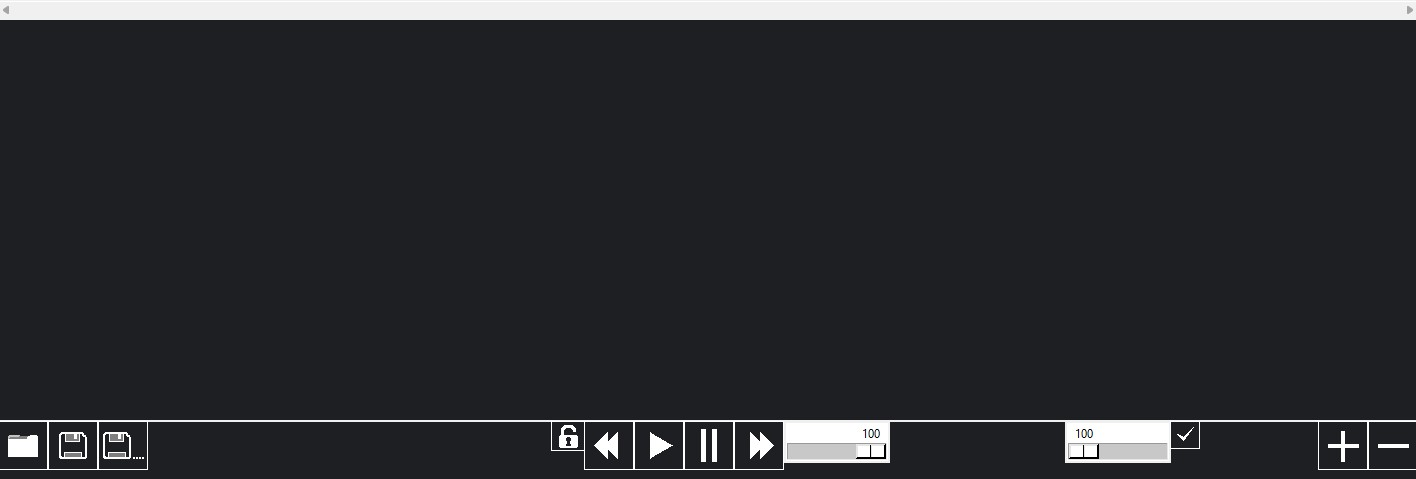
\includegraphics[width=1\linewidth]{test_case1}}
\caption{Аудиодорожка до загрузки аудиофайла}
\label{test_case:image}
\end{figure}

\begin{figure}[H] 
	\center{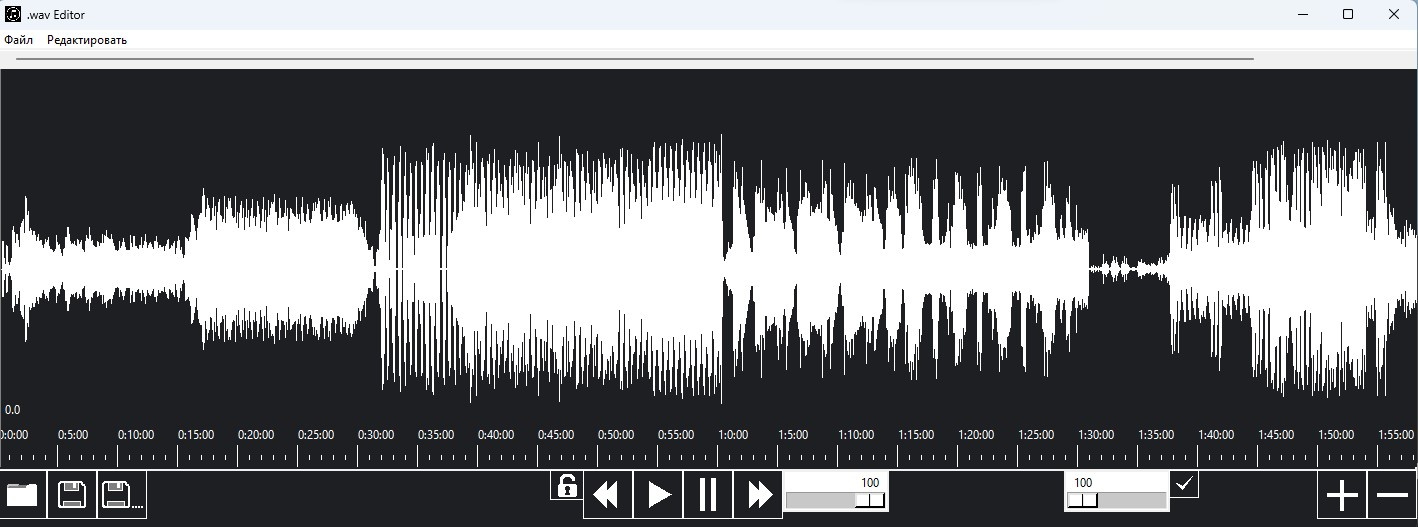
\includegraphics[width=1\linewidth]{test_case2}}
	\caption{Аудиодорожка после загрузки аудиофайла}
	\label{test_case1:image}
\end{figure}

\subsubsection{Проигрыввание аудио}
Предусловие: програма запущена, аудиофайл загружен.

Тестовый случай: проигрывание аудио.

Ожидаемый результат: корректное воспроизведение аудиоданных.

Результат представлен на рисунках \ref{test_case2:image} и \ref{test_case3:image}.

\begin{figure}[H]
	\center{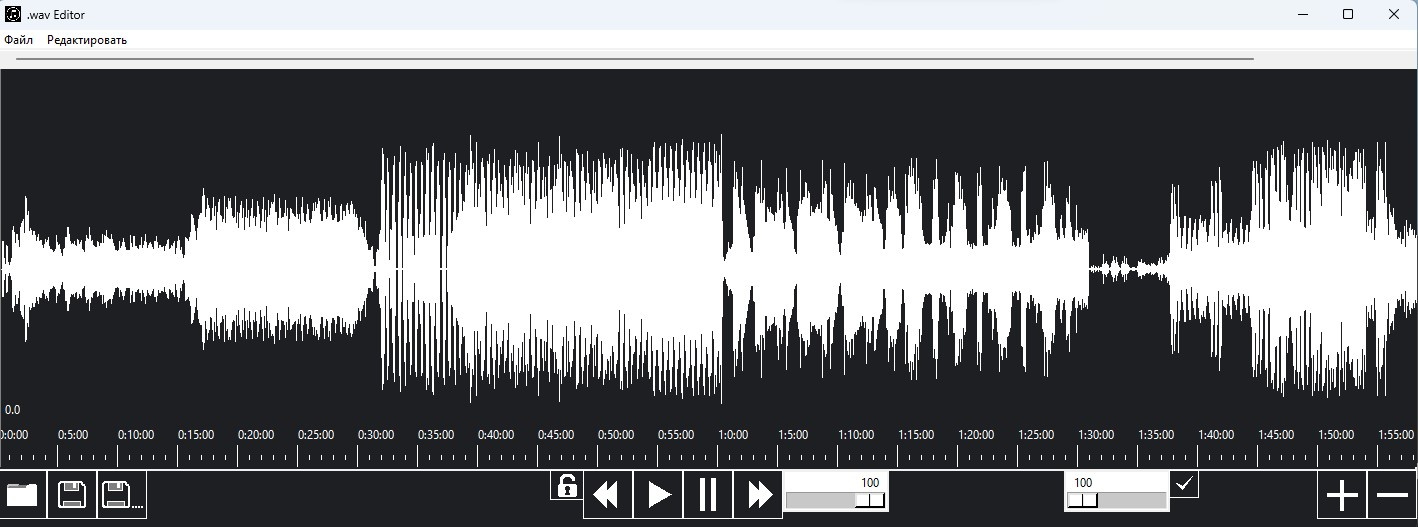
\includegraphics[width=1\linewidth]{test_case2}}
	\caption{Аудиодорожка до воспроизведения аудиофайла}
	\label{test_case2:image}
\end{figure}

\begin{figure}[H] 
	\center{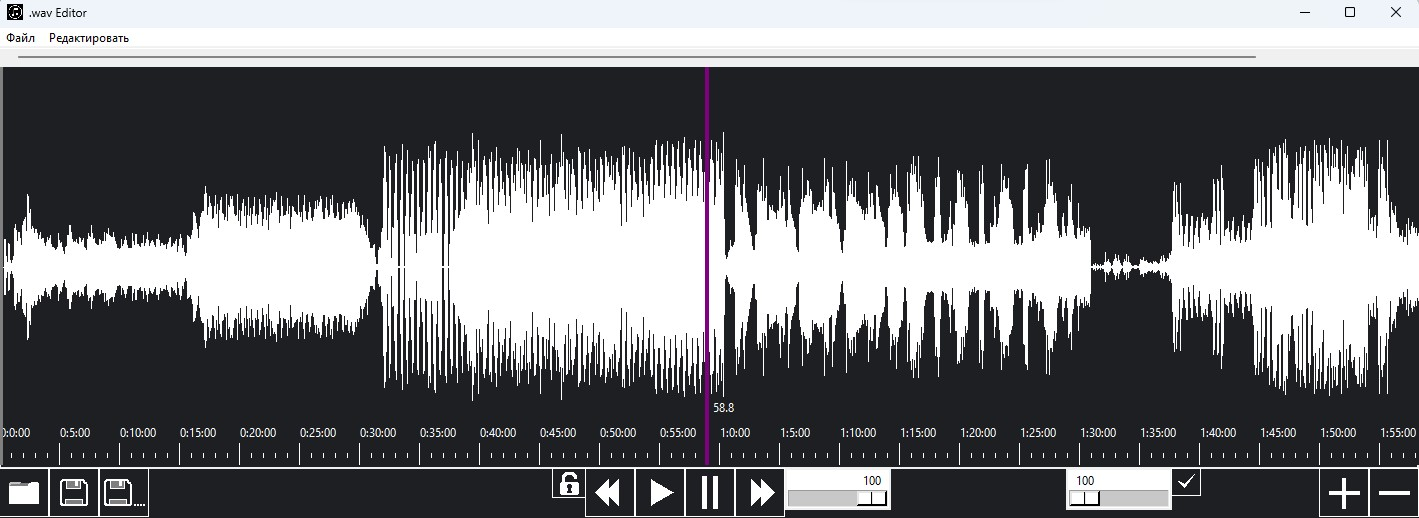
\includegraphics[width=1\linewidth]{test_case3}}
	\caption{Аудиодорожка после воспроизведения аудиофайла}
	\label{test_case3:image}
\end{figure}

\subsubsection{Выделение области}
Предусловие: програма запущена, аудиофайл загружен.

Тестовый случай: выделение области аудио.

Ожидаемый результат: корректное выделение области.

Результат представлен на рисунках \ref{test_case5:image} и \ref{test_case6:image}.

\begin{figure}[H]
	\center{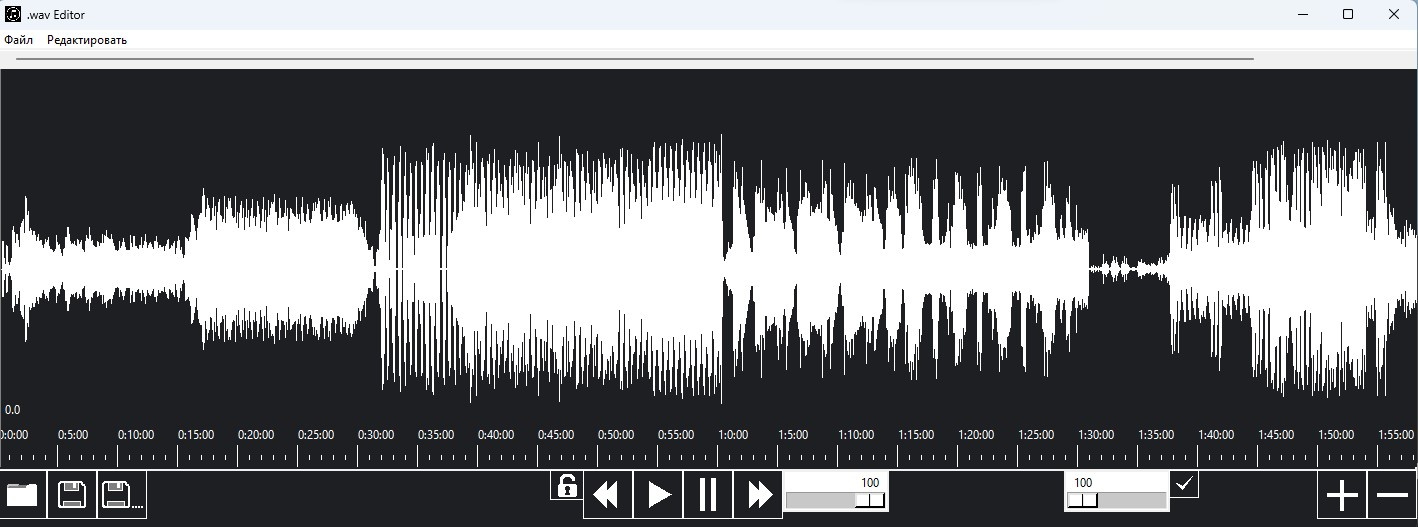
\includegraphics[width=1\linewidth]{test_case2}}
	\caption{Аудиодорожка до выбора области}
	\label{test_case5:image}
\end{figure}

\begin{figure}[H] 
	\center{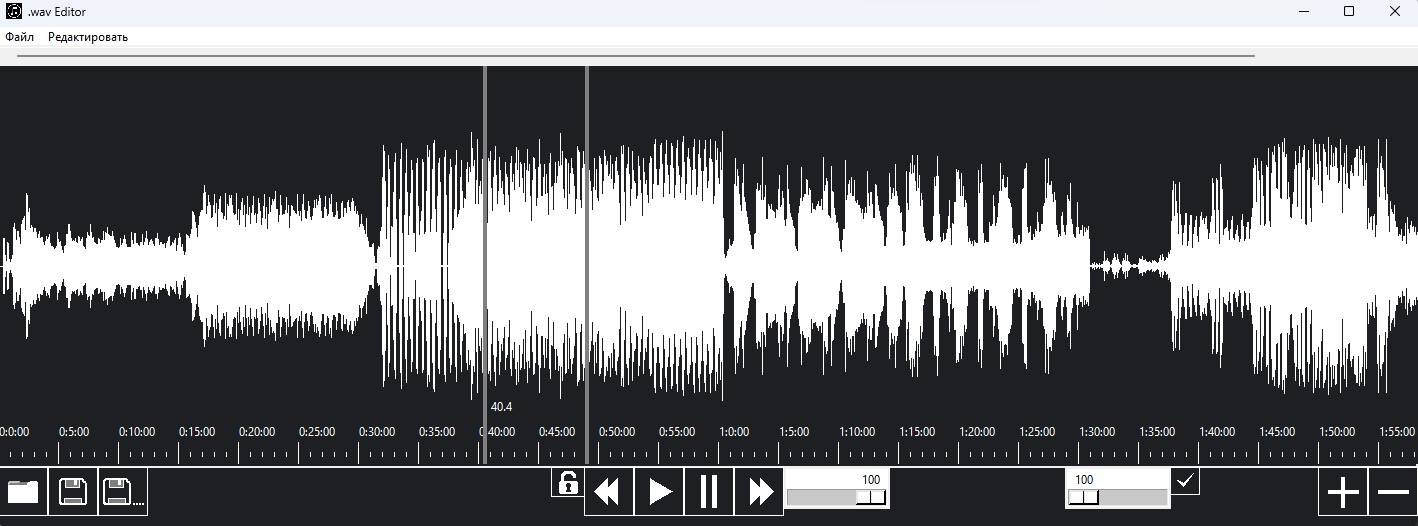
\includegraphics[width=1\linewidth]{test_case4}}
	\caption{Аудиодорожка после выбора области}
	\label{test_case6:image}
\end{figure}

\subsubsection{Редактирование аудиоданных}
Предусловие: програма запущена, аудиофайл загружен, выбрана необходимая область.

Тестовый случай: удаление области.

Ожидаемый результат: корректное удаление области.

Результат представлен на рисунках \ref{test_case7:image} и \ref{test_case8:image}.

\begin{figure}[H]
	\center{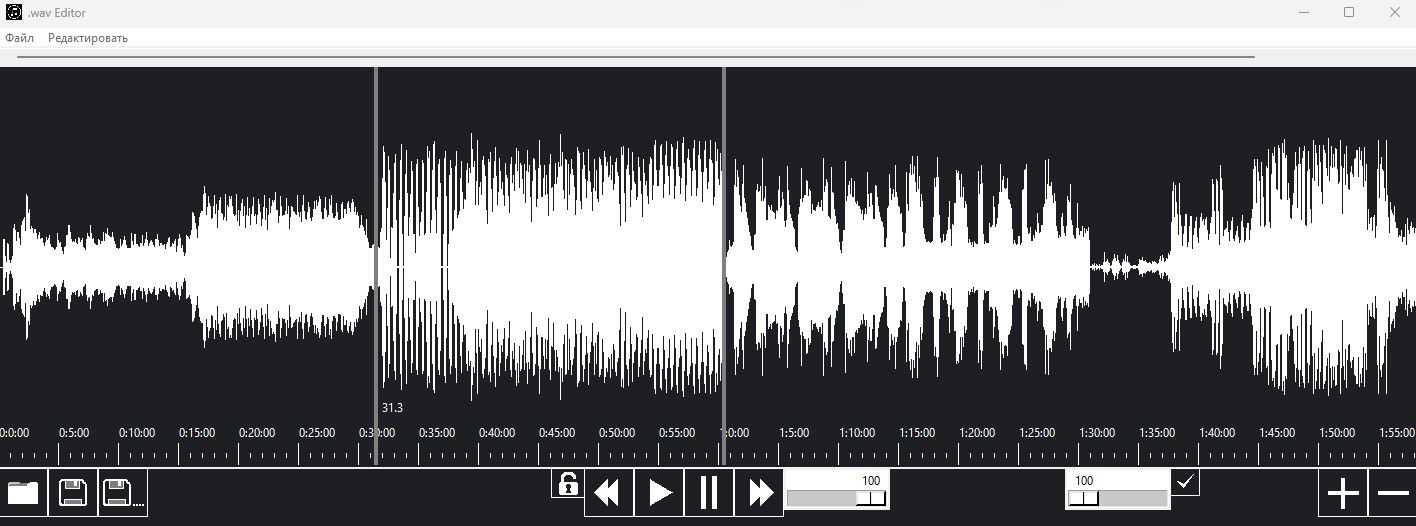
\includegraphics[width=1\linewidth]{test_case5}}
	\caption{Аудиодорожка до удаления области}
	\label{test_case7:image}
\end{figure}

\begin{figure}[H] 
	\center{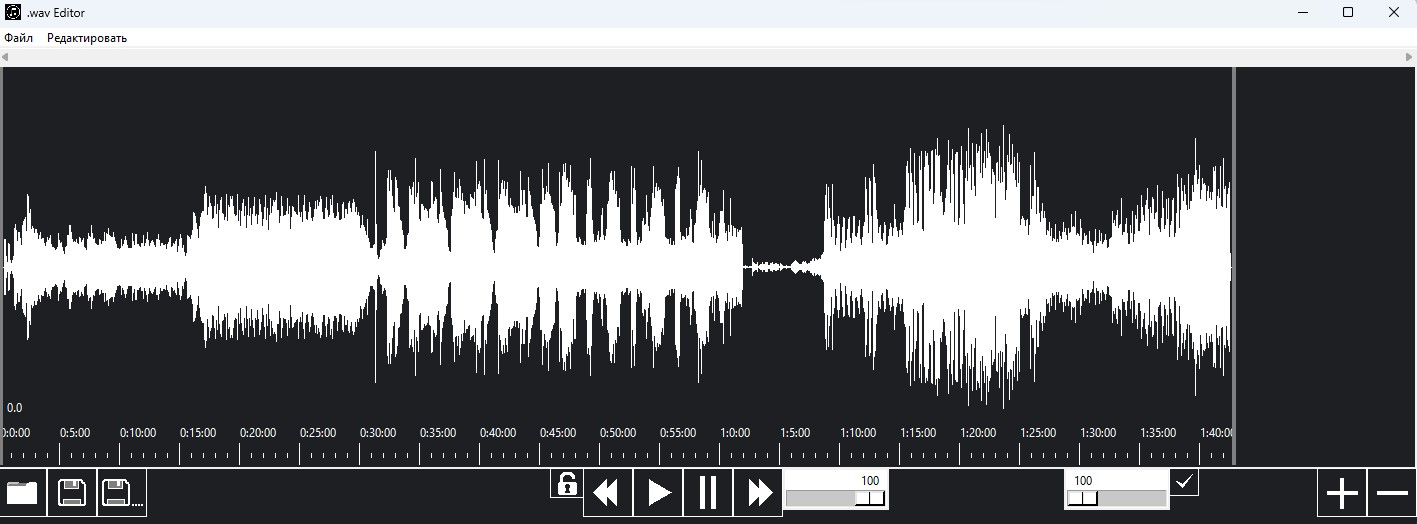
\includegraphics[width=1\linewidth]{test_case6}}
	\caption{Аудиодорожка после удаления области}
	\label{test_case8:image}
\end{figure}

Предусловие: програма запущена, аудиофайл загружен, скопирована вставляемая область.

Тестовый случай: вставка области.

Ожидаемый результат: корректная вставка области.

Результат представлен на рисунках \ref{test_case9:image} и \ref{test_case10:image}.

\begin{figure}[H]
	\center{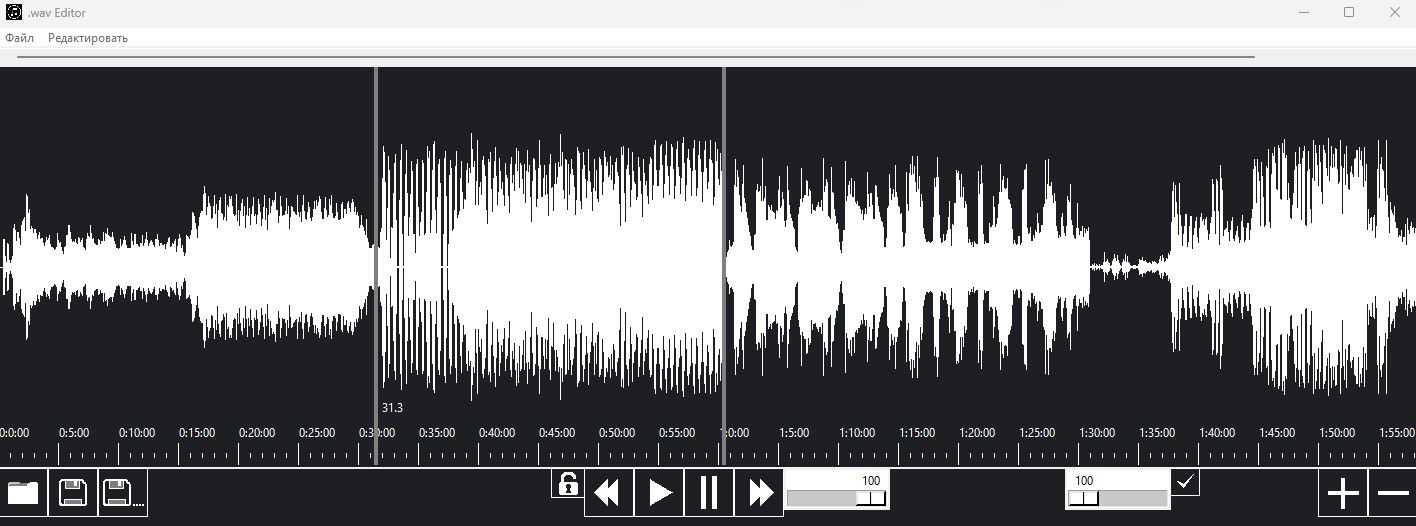
\includegraphics[width=1\linewidth]{test_case5}}
	\caption{Аудиодорожка до вставки области}
	\label{test_case9:image}
\end{figure}

\begin{figure}[H] 
	\center{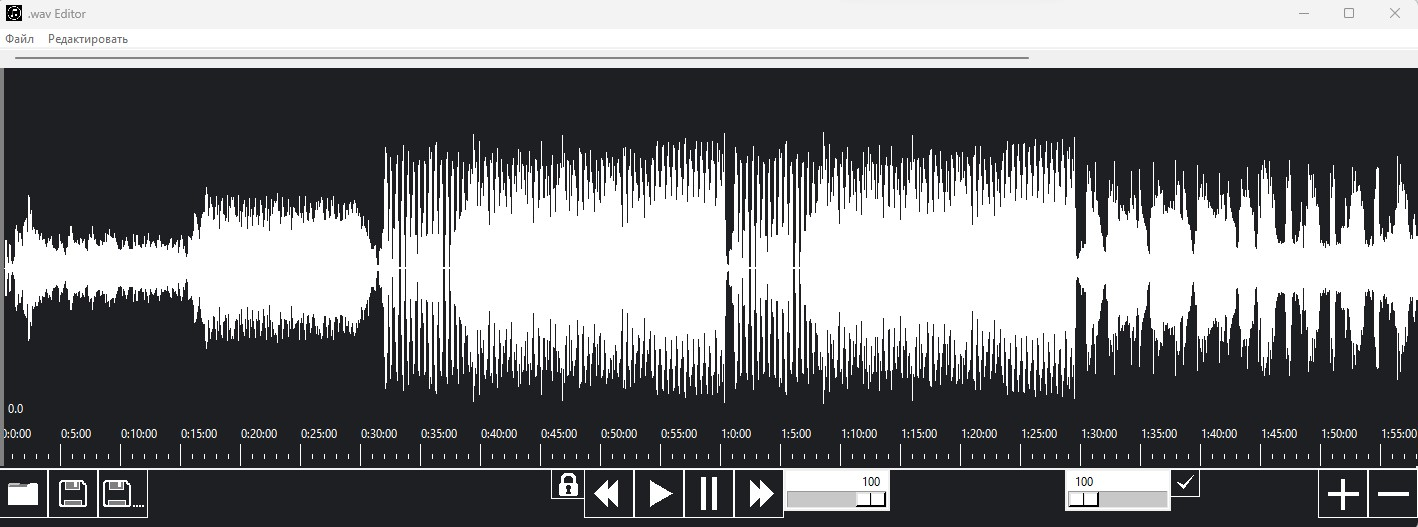
\includegraphics[width=1\linewidth]{test_case7}}
	\caption{Аудиодорожка после вставки области}
	\label{test_case10:image}
\end{figure}

Предусловие: програма запущена, аудиофайл загружен, скопирована замещающая и выбрана заменяемая области.

Тестовый случай: вставка области.

Ожидаемый результат: корректная замена области.

Результат представлен на рисунках \ref{test_case11:image} и \ref{test_case12:image}.

\begin{figure}[H]
	\center{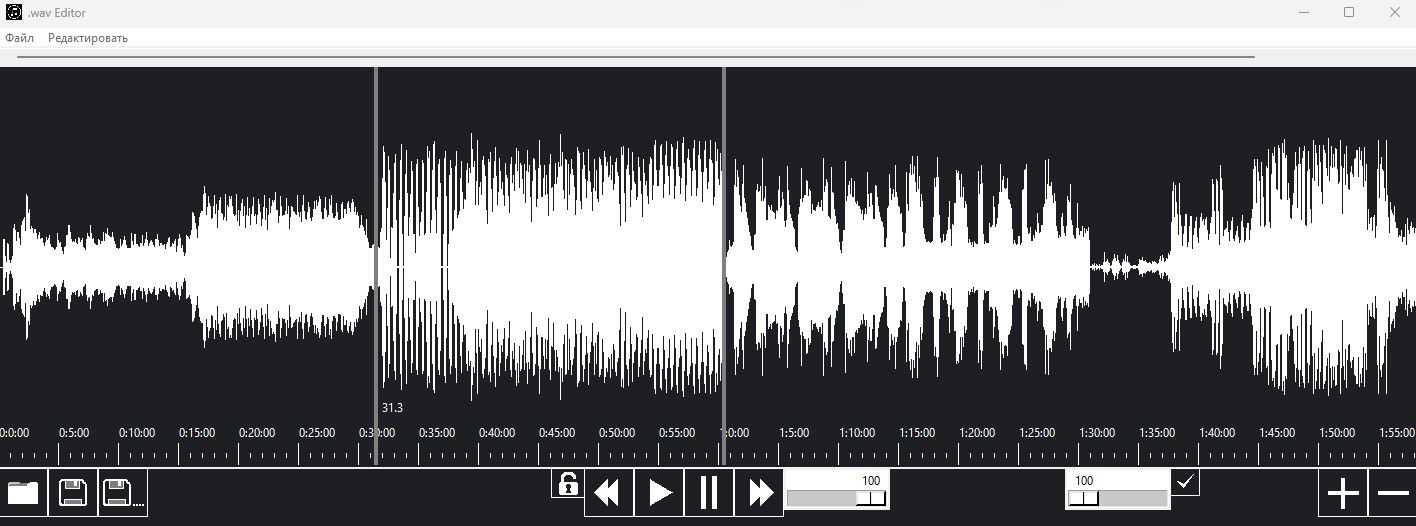
\includegraphics[width=1\linewidth]{test_case5}}
	\caption{Аудиодорожка до замены области}
	\label{test_case11:image}
\end{figure}

\begin{figure}[H] 
	\center{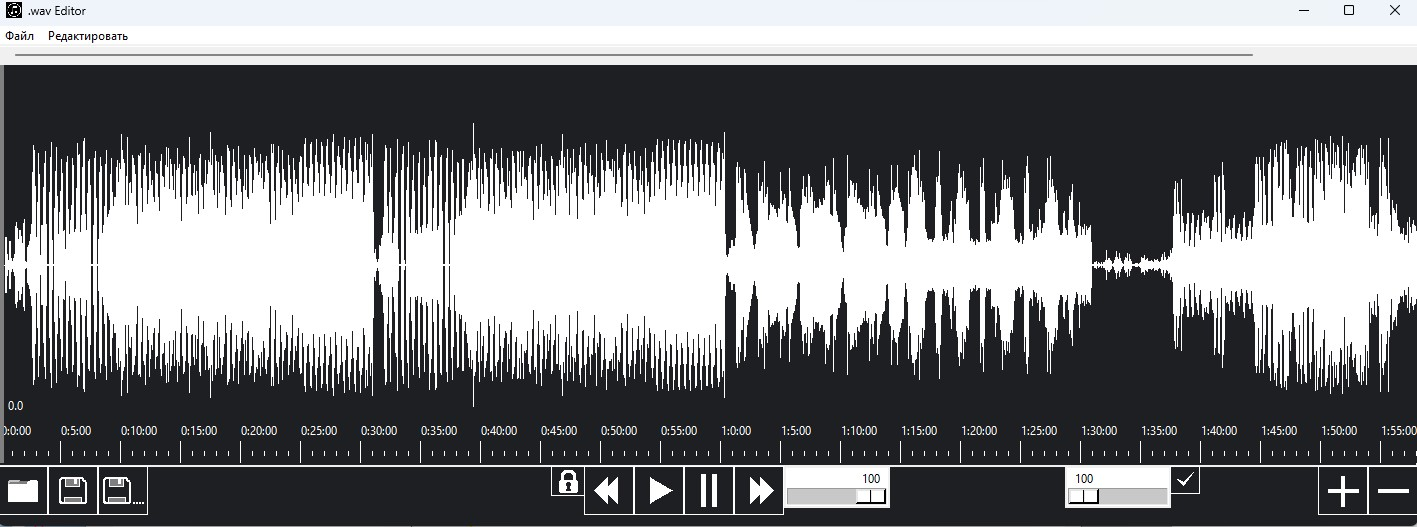
\includegraphics[width=1\linewidth]{test_case8}}
	\caption{Аудиодорожка после замены области}
	\label{test_case12:image}
\end{figure}

Предусловие: програма запущена, аудиофайл загружен, выбрана необходимая область.

Тестовый случай: обнуление области.

Ожидаемый результат: корректное обнуление области.

Результат представлен на рисунках \ref{test_case13:image} и \ref{test_case14:image}.

\begin{figure}[H]
	\center{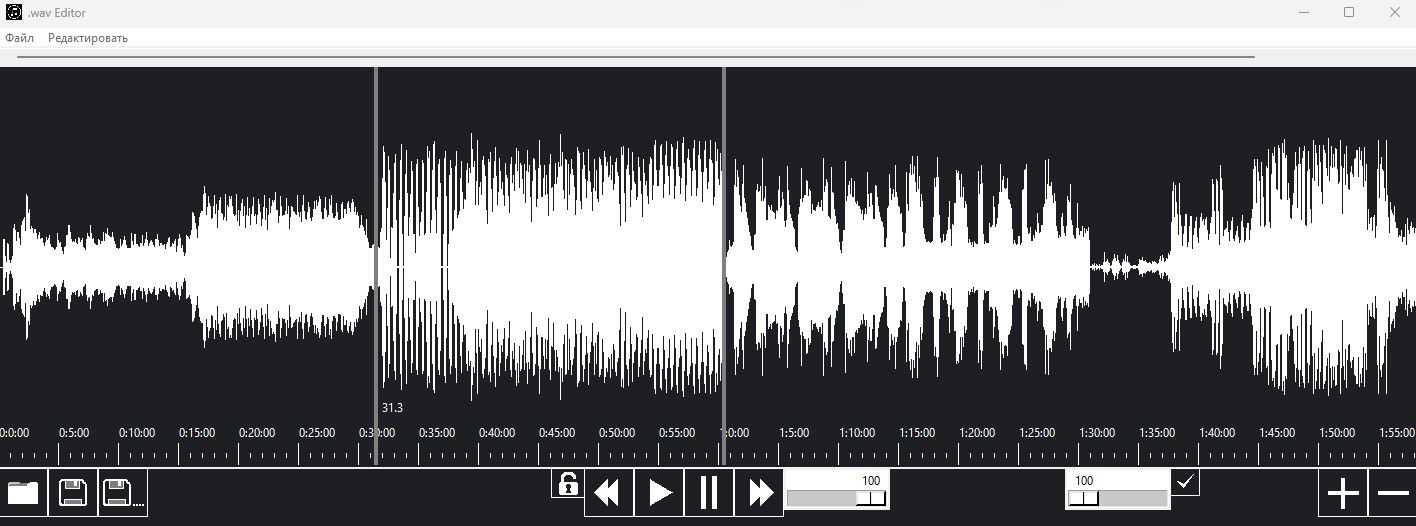
\includegraphics[width=1\linewidth]{test_case5}}
	\caption{Аудиодорожка до обнуления области}
	\label{test_case13:image}
\end{figure}

\begin{figure}[H] 
	\center{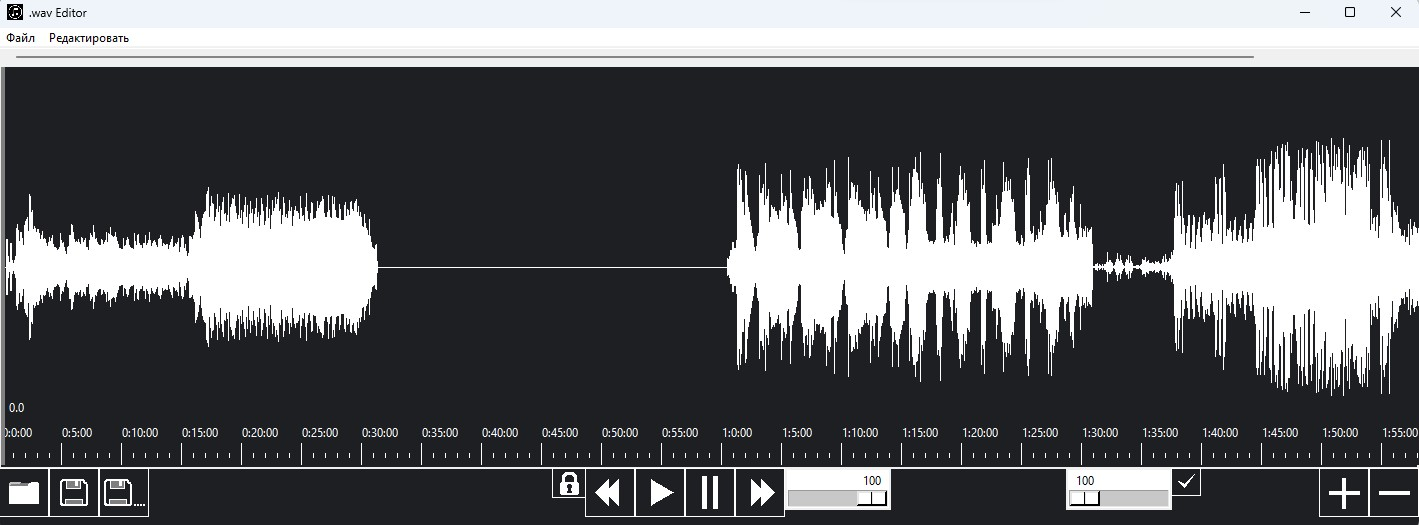
\includegraphics[width=1\linewidth]{test_case9}}
	\caption{Аудиодорожка после обнуления области}
	\label{test_case14:image}
\end{figure}

Предусловие: програма запущена, аудиофайл загружен, выбрана необходимая область.

Тестовый случай: нарастание области.

Ожидаемый результат: корректное применение эффекта нарастания области.

Результат представлен на рисунках \ref{test_case15:image} и \ref{test_case16:image}.

\begin{figure}[H]
	\center{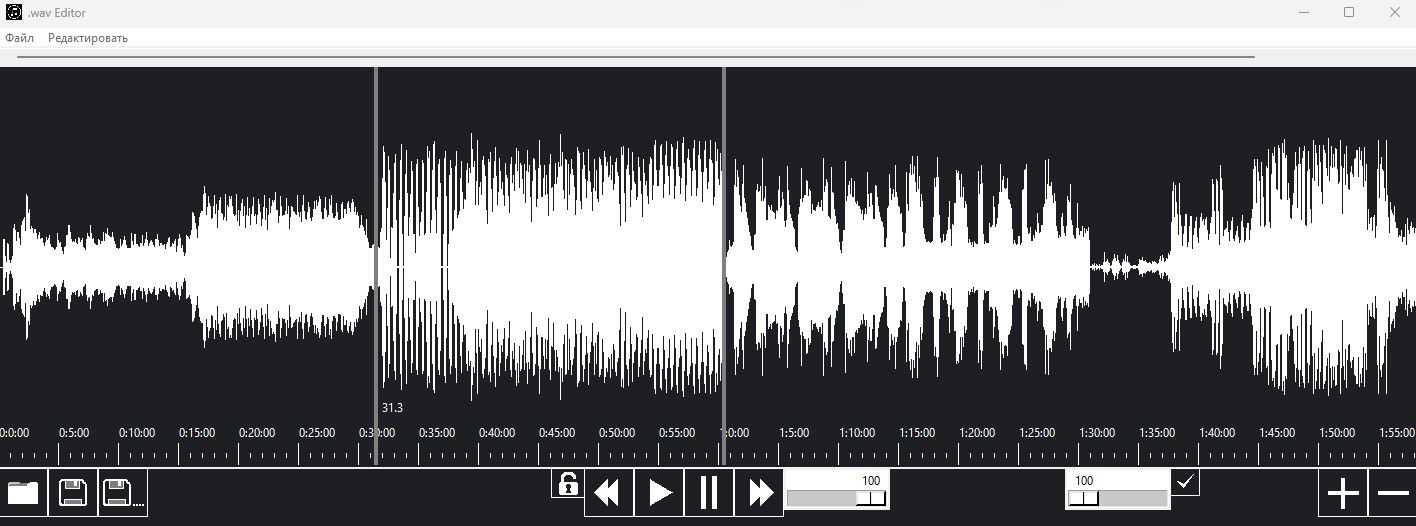
\includegraphics[width=1\linewidth]{test_case5}}
	\caption{Аудиодорожка до применения эффекта}
	\label{test_case15:image}
\end{figure}

\begin{figure}[H] 
	\center{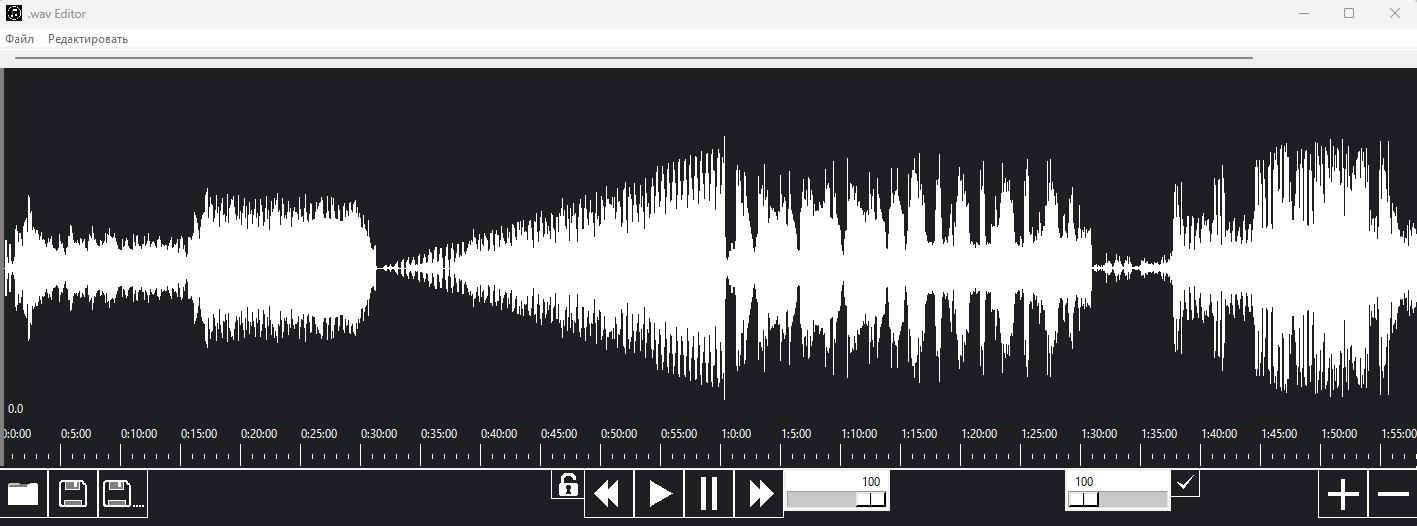
\includegraphics[width=1\linewidth]{test_case10}}
	\caption{Аудиодорожка после применения эффекта}
	\label{test_case16:image}
\end{figure}

Предусловие: програма запущена, аудиофайл загружен, выбрана необходимая область.

Тестовый случай: затухание области.

Ожидаемый результат: корректное применение эффекта затухания области.

Результат представлен на рисунках \ref{test_case17:image} и \ref{test_case18:image}.

\begin{figure}[H]
	\center{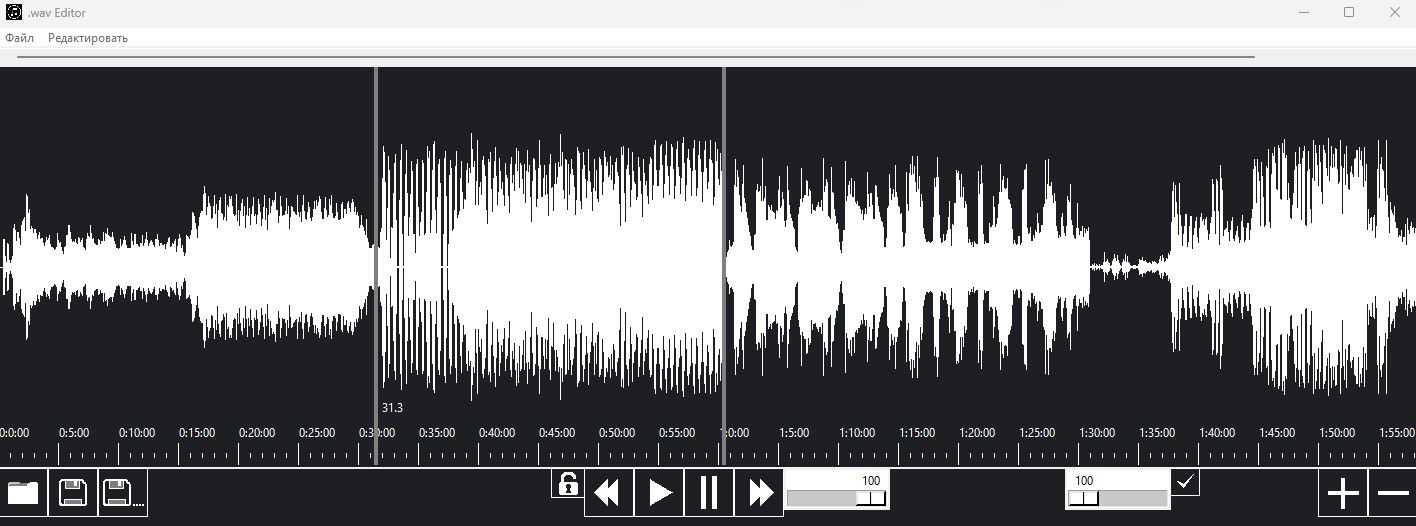
\includegraphics[width=1\linewidth]{test_case5}}
	\caption{Аудиодорожка до применения эффекта}
	\label{test_case17:image}
\end{figure}

\begin{figure}[H] 
	\center{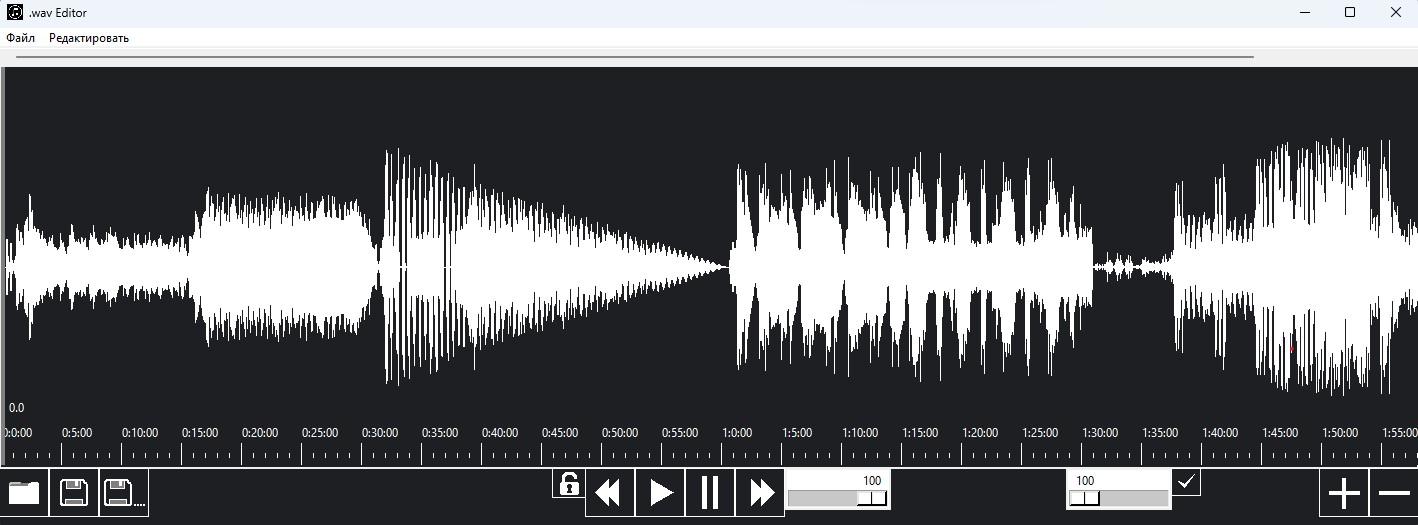
\includegraphics[width=1\linewidth]{test_case11}}
	\caption{Аудиодорожка после применения эффекта}
	\label{test_case18:image}
\end{figure}

\subsubsection{Управление действиями}

Предусловие: програма запущена, аудиофайл загружен, совершенно какое-либо изменение аудиоданных.

Тестовый случай: отмена операции.

Ожидаемый результат:  корректная отмена совершенной операции.

Результат представлен на рисунках \ref{test_case19:image} и \ref{test_case20:image}.

\begin{figure}[H]
	\center{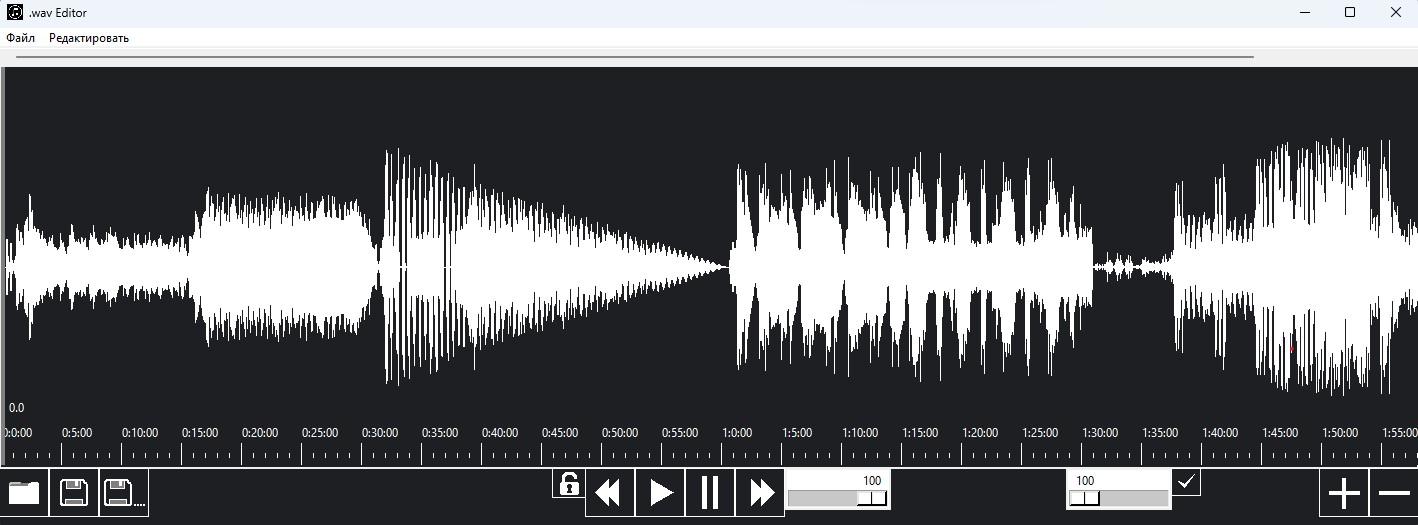
\includegraphics[width=1\linewidth]{test_case11}}
	\caption{Аудиодорожка до отмены операции}
	\label{test_case19:image}
\end{figure}

\begin{figure}[H] 
	\center{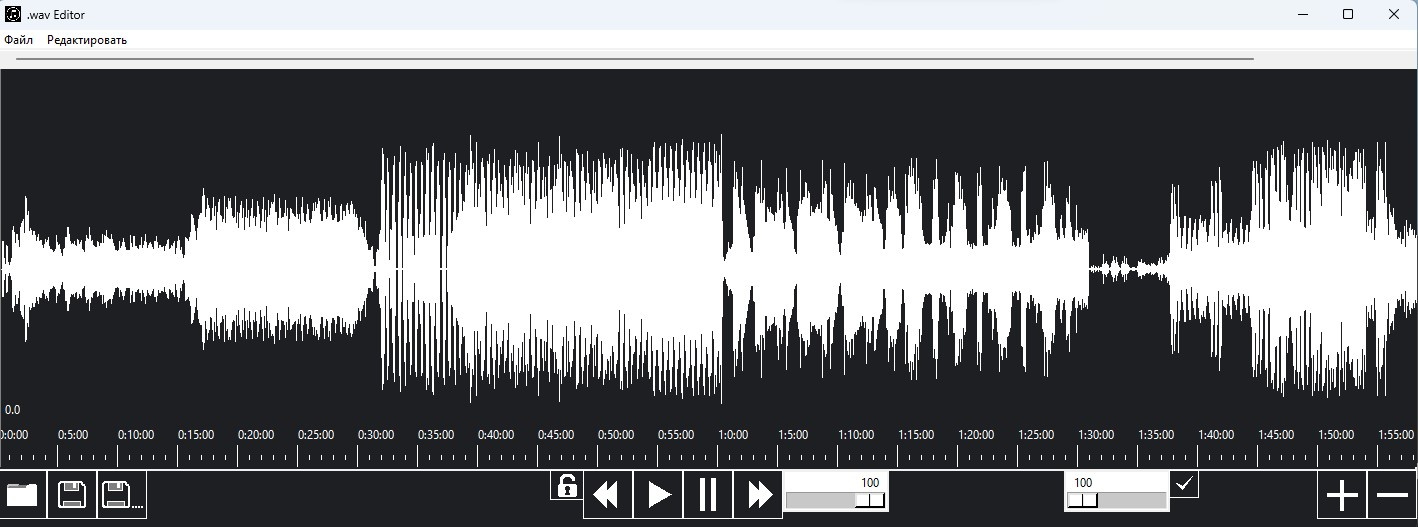
\includegraphics[width=1\linewidth]{test_case2}}
	\caption{Аудиодорожка после отмены операции}
	\label{test_case20:image}
\end{figure}

Предусловие: програма запущена, аудиофайл загружен, совершенно какое-либо изменение аудиоданных.

Тестовый случай: возврат операции.

Ожидаемый результат: корректный возврат совершенной операции.

Результат представлен на рисунках \ref{test_case21:image} и \ref{test_case22:image}.

\begin{figure}[H]
	\center{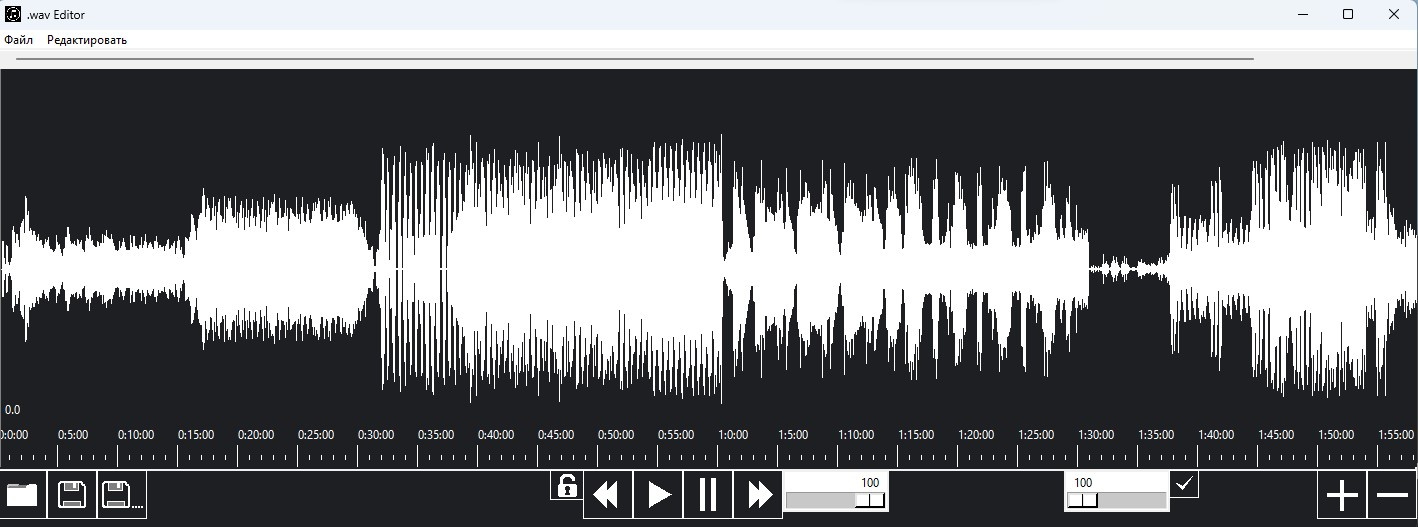
\includegraphics[width=1\linewidth]{test_case2}}
	\caption{Аудиодорожка до возврата операции}
	\label{test_case21:image}
\end{figure}

\begin{figure}[H] 
	\center{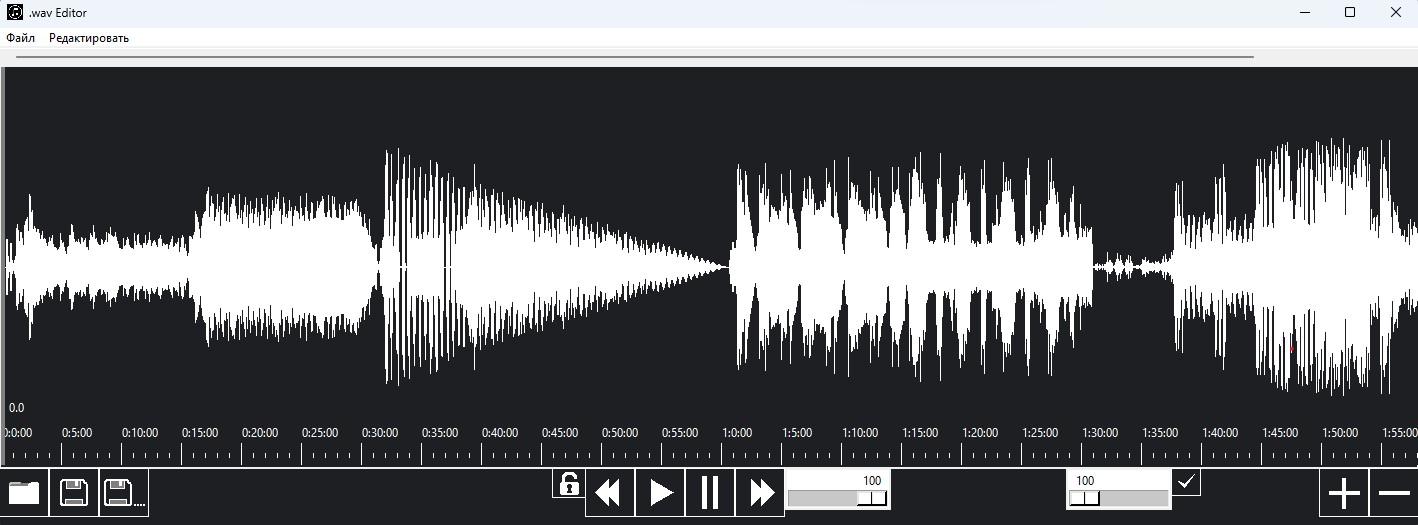
\includegraphics[width=1\linewidth]{test_case11}}
	\caption{Аудиодорожка после возврата операции}
	\label{test_case22:image}
\end{figure}

\subsubsection{Сохранение аудиофайла}

Предусловие: програма запущена, аудиофайл загружен, совершенны какие-либо операции над аудиоданными (необязательно).

Тестовый случай: сохранение аудиофайла.

Ожидаемый результат: корректное сохранение аудиофайла.

Результат представлен на рисунках \ref{test_case23:image} и \ref{test_case24:image}.

\begin{figure}[H]
	\center{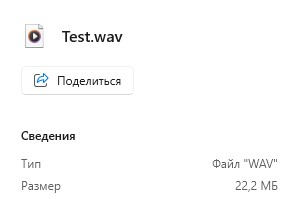
\includegraphics[width=0.5\linewidth]{test_case12}}
	\caption{Размер оригинального аудиофайла}
	\label{test_case23:image}
\end{figure}

\begin{figure}[H] 
	\center{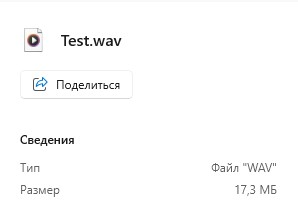
\includegraphics[width=0.5\linewidth]{test_case13}}
	\caption{Размер аудиофайла после сохранения с изменениями}
	\label{test_case24:image}
\end{figure}